\documentclass{beamer}

\usetheme{simple}

\usepackage{scalerel,xparse}
\usepackage{lmodern}
\usepackage[scale=2]{ccicons}
\usepackage{ulem}
\usepackage{tikz}
\usetikzlibrary{positioning,calc,automata}
\usepackage{algorithm}
\usepackage{algorithmic}
\usepackage{caption}
\usepackage{listings}
\usepackage{xcolor}

% Watermark background (simple theme)
\setlength{\parindent}{0cm}
\setwatermark{
\includegraphics[height=8cm]{img/chungus_pekora.png}}

\NewDocumentCommand\emojisushi{}{
    
\includegraphics{img/1f363.png}
}
\NewDocumentCommand\emojimoyai{}{
    
\includegraphics{img/1f5ff.png}
}   
\NewDocumentCommand\emojicarrot{}{
    
\includegraphics[width=0.3cm]{img/1f955.png}
}   
\NewDocumentCommand\emojiflushed{}{
    
\includegraphics[width=0.3cm]{img/1f633.png}
}   

\title{CSC363 Tutorial 8}
\subtitle{What does P stand for?}
\date{\today}
\author{Paul ``sushi{\textunderscore}enjoyer'' Zhang}
\institute{University of Humongus Chungus Amogus Pekora\emojicarrot}

\begin{document}

\maketitle

\begin{frame}{What does P stand for?}
P stands for \textbf{Practical!}\footnote{not really. some problems that we think are not in P are still of practical importance! for example, the \textbf{Travelling Salesman Problem (TSP)} is believed to not be in P, yet we need it for stuff like, uh, sushi delivery? \emojisushi \emojisushi}

\vspace{2mm}

\pause

Not really. P stands for \textit{polynomial-time}. It is formally defined as $$ \text P = \bigcup_{k = 1}^\infty \text{TIME}(n^k)$$
where $\text{TIME}(n^k)$ is the set of languages that can be decided by a $O(n^k)$ TM.

\vspace{2mm}

\pause

Less formally, P is the set of languages that can be decided by a poly-time TM.

\vspace{2mm}

Remember: just because \textit{some} algorithm for deciding a language $A$ isn't poly-time does not mean \textit{all} algorithms for deciding $A$ aren't poly-time.
\end{frame}

\begin{frame}{Learning objectives this tutorial}
By the end of this tutorial, you should...
\begin{itemize}
\item Remove \url{turingmachinesimulator.com} from your bookmarks in Microsoft Edge (or whichever browser you use), cuz we are past the low-level Turing machine stuff :(
\item Watch the video on P vs NP pinned on Piazza, if you haven't yet!
\item Have a brief image of the ``computability hierarchy'' in the back of your head.
\item Understand what NP means. Now you get to explain the P = NP problem to your friends and be a cool person or something smh.
\end{itemize}
\texttt{helo\textunderscore fish.jpg} certified readings: 7.1-7.3, probably, in Sipser's book.
\end{frame}

\begin{frame}{When Turing machine is sus \emojiflushed \emojiflushed}

A non-deterministic Turing machine takes the next CSC363 quiz. It \textit{chooses} the correct answers.

\vspace{2mm}

A non-deterministic Turing machine forgets its bank account password. It \textit{chooses} the correct password.

\vspace{2mm}

A non-deterministic Turing machine plays the hit game \textit{amogus}. It \textit{chooses} the imposter to vote out.

\vspace{2mm}

\pause

Recall (i'm not sure if you do, from the tutorial 2 weeks ago, but meh): we say a non-deterministic turing machine accepts an input if and only if there is \textit{some} execution path for the NTM that results in acceptance.

\vspace{2mm}

Unfortunately, there isn't any \url{nondeterministicturingmachinesimulator.com} out there (unless you want to create it!). 

\end{frame}

\begin{frame}{H-path}
\textbf{Task:} Guess what the H stands for in HPATH. I'll actually give you 0.2 bonus marks on your next assignment if you know the answer.

\pause

\textbf{Answer:} H stands for \textit{Hamilton}. Not from Ontario. Hamilton is this Irish lad:

\begin{figure}[h]
\centering
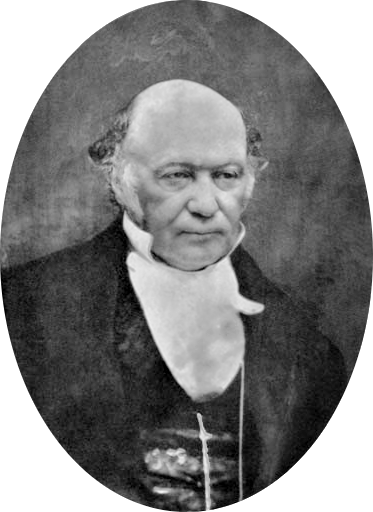
\includegraphics[height=5cm]{img/hamilton.png}
\caption*{helo}
\end{figure}


\end{frame}

\begin{frame}{H-path}
{\tiny sowwy, tikz is too tedious ;-; you'll have to refer to my hand drawn graphs instead.}

\begin{columns}
\column{0.4\linewidth}
\begin{figure}[h]
\centering
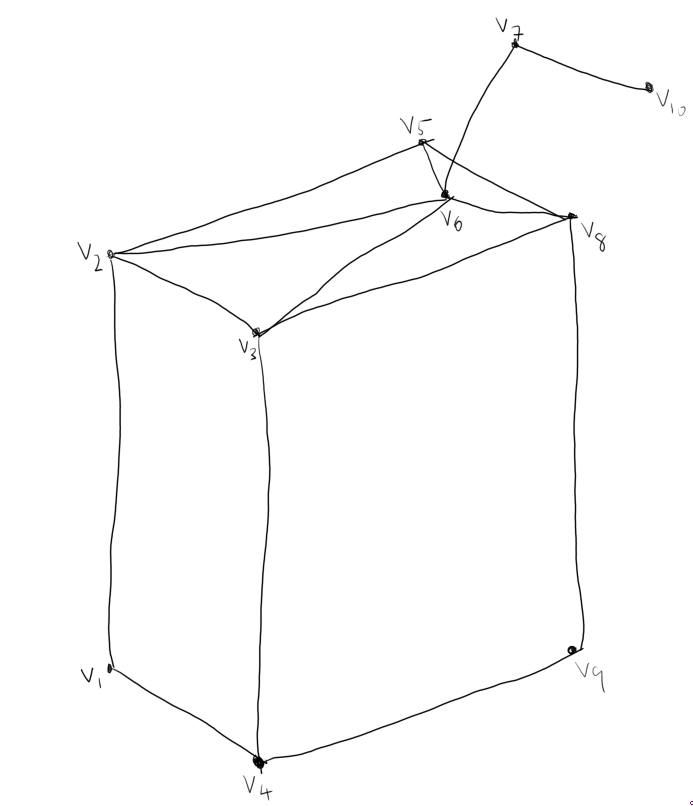
\includegraphics[height=6cm]{img/graph_juice.png}
\end{figure}
\column{0.5\linewidth}

Given an (undirected) graph, a \textbf{Hamiltonian path} is a path that visits each vertex \textit{exactly once}. The \textbf{Hamiltonian path problem} asks you to determine if a Hamiltonian path exists given an arbitrary graph.


\vspace{4mm}

\textbf{Task:} Is there a Hamiltonian path in this graph?
\end{columns}




\end{frame}

\begin{frame}{H-path}
{\tiny sowwy, tikz is too tedious ;-; you'll have to refer to my hand drawn graphs instead.}

\begin{columns}
\column{0.4\linewidth}
\begin{figure}[h]
\centering
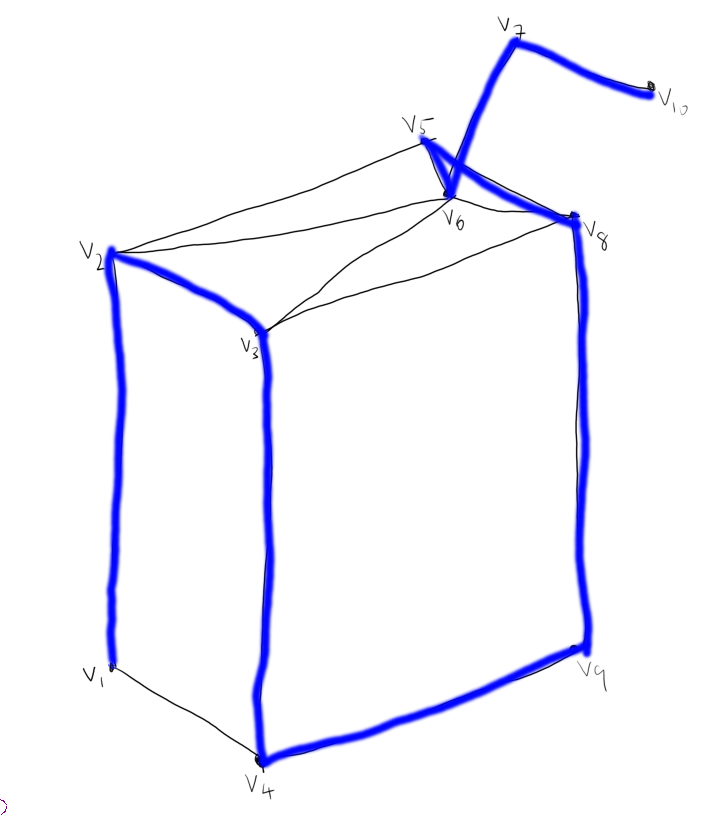
\includegraphics[height=6cm]{img/graph_juice_path.png}
\end{figure}
\column{0.5\linewidth}

\textbf{Answer:} yes! consider the path\\ $v_1$, $v_2$, $v_3$ $v_4$, $v_9$, $v_8$, $v_5$, $v_6$, $v_7$, $v_{10}$.
\end{columns}
\end{frame}

\begin{frame}{H-path}
{\tiny sowwy, tikz is too tedious ;-; you'll have to refer to my hand drawn graphs instead.}

\begin{figure}[h]
\centering
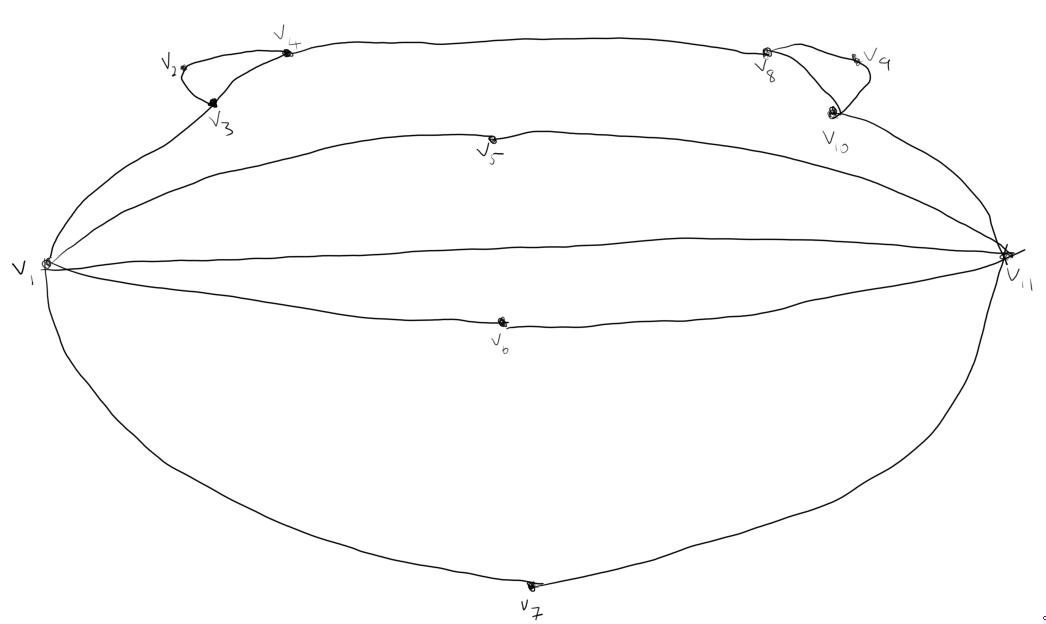
\includegraphics[height=6cm]{img/graph_helo.png}
\end{figure}

\textbf{Task:} Is there a Hamiltonian path in this graph?

\pause

\textbf{Answer:} No. (I've checked every possible Hamiltonian path).

\end{frame}

\begin{frame}{H-path}
Here's a deterministic TM $M$ to check if there is a H-path, given a graph input $G$:
\begin{align*}
M(G): &\text{Let $v_1, v_2, \ldots, v_n$ be the vertices of $G$}\\
&\text{For every permutation $P$ of $[v_1, v_2, \ldots, v_n]$:}\\
&\quad \text{If $P$ is a valid path in $G$:}\\
&\quad \quad \text{Accept}\\
&\text{Reject}
\end{align*}

But this is very inefficient, and you probably wouldn't try this on an interview.

\textbf{Task:} Convince yourself that the above algorithm takes at least $n!$ time, where $n$ is the size of the input (the number of vertices in our graph). So the above algorithm is not polynomial time.

\textbf{Task:}\footnote{Don't actually try this.} Design a poly-time algorithm that solves the H-path problem. Send it to me. I'll give you a 10\% bonus in this course.

\end{frame}

\begin{frame}{H-path}
Here's a non-deterministic Turing machine $M$ to check if there is a H-path, given a graph input $G$:
\begin{align*}
M(G):& \text{Let $v_1, v_2, \ldots, v_n$ be the vertices of $G$}\\
&\text{Nondeterministically \textit{choose} a permutation $P$ of $[v_1, v_2, \ldots, v_n]$}\\
&\text{If $P$ is a valid path in $G$:}\\
&\quad \text{Accept}\\
&\text{Reject}
\end{align*}

\textbf{Task:} Ask yourself, ``Why does $M$ accept input $G$ if and only if $G$ has a Hamiltonian path?'' 

\end{frame}

\begin{frame}{H-path}

We've said that the \textbf{running time} of a deterministic TM $M$ is the function $f(n)$ such that 
$$f(n) = \max\{s: \text{$M(x)$ halts in exactly $s$ steps, $|x| = n$}\}$$

We'll define the \textbf{running time} of a non-deterministic TM $M$ to be the function
$$f(n) = \max\{s: \text{\small for some execution path, $M(x)$ halts in exactly $s$ steps, $|x| = n$}\}$$

In other words, $f(n)$ is the maximum time it will take to halt over all input of length $n$ and all execution paths.

\begin{figure}[h]
\centering
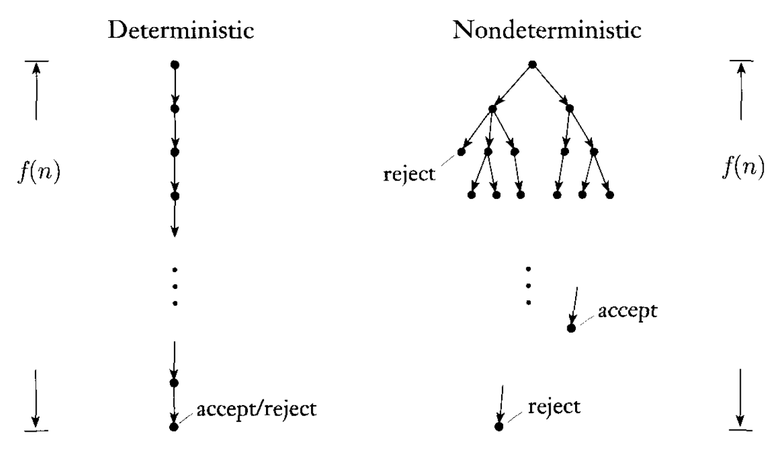
\includegraphics[width=5cm]{img/copied_diagram}
\caption*{pls dont sue me google images}
\end{figure}

\end{frame}

\begin{frame}{H-path}

Define $\text{NTIME}(f(n))$ to be the set of languages $A$ such that there is a $O(f(n))$ non-deterministic Turing machine that decides $A$.

Define $$\text{NP} = \bigcup_{k = 1}^\infty \text{NTIME}(n^k).$$
In other words, NP is the set of languages that have poly-time NTM deciders.

\vspace{2mm}

Now you can tell your friends about the P vs NP problem!

\textbf{Task:} Show $\text P \subseteq \text{NP}$.

\pause
\textbf{Answer:} Every poly-time TM is also a nondeterministic poly-time TM (except it only has one possible execution path). So for any language $A$ in P, a poly-time decider for $A$ would also be a non-deterministic poly-time decider for $A$, so $A \in \text{NP}$.

\end{frame}


\begin{frame}{H-path}

\begin{align*}
M(G):& \text{Let $v_1, v_2, \ldots, v_n$ be the vertices of $G$}\\
&\text{Nondeterministically \textit{choose} a permutation $P$ of $[v_1, v_2, \ldots, v_n]$}\\
&\text{If $P$ is a valid path in $G$:}\\
&\quad \text{Accept}\\
&\text{Reject}
\end{align*}

\textbf{Task:} Convince yourself that the above non-deterministic Turing machine takes polynomial time to halt, given a graph $G$ of $n$ vertices. Conclude that the following language is in NP:

$$\text{HPATH} = \{G: \text{$G$ is a graph with a Hamiltonian path}\}.$$

(we actually don't know if the above language is in P! that would actually amount to proving P $=$ NP.)

\end{frame}

\begin{frame}{sushi juice, part 2.}
\begin{figure}[h]
\centering

\includegraphics[width=5cm]{img/helo_fish_sushi.jpg}
\end{figure}

\textbf{Task:} Guess what I've ate today.

\pause

\textbf{Task:} Guess what is in this ``juice''.

\pause

\textbf{Task:} Guess who was feeling sadistic while designing Assignment 4.

\end{frame}


\begin{frame}{here's a zoo.}
We'll call it the \textit{computational complexity zoo}.

\begin{figure}[h]
\centering
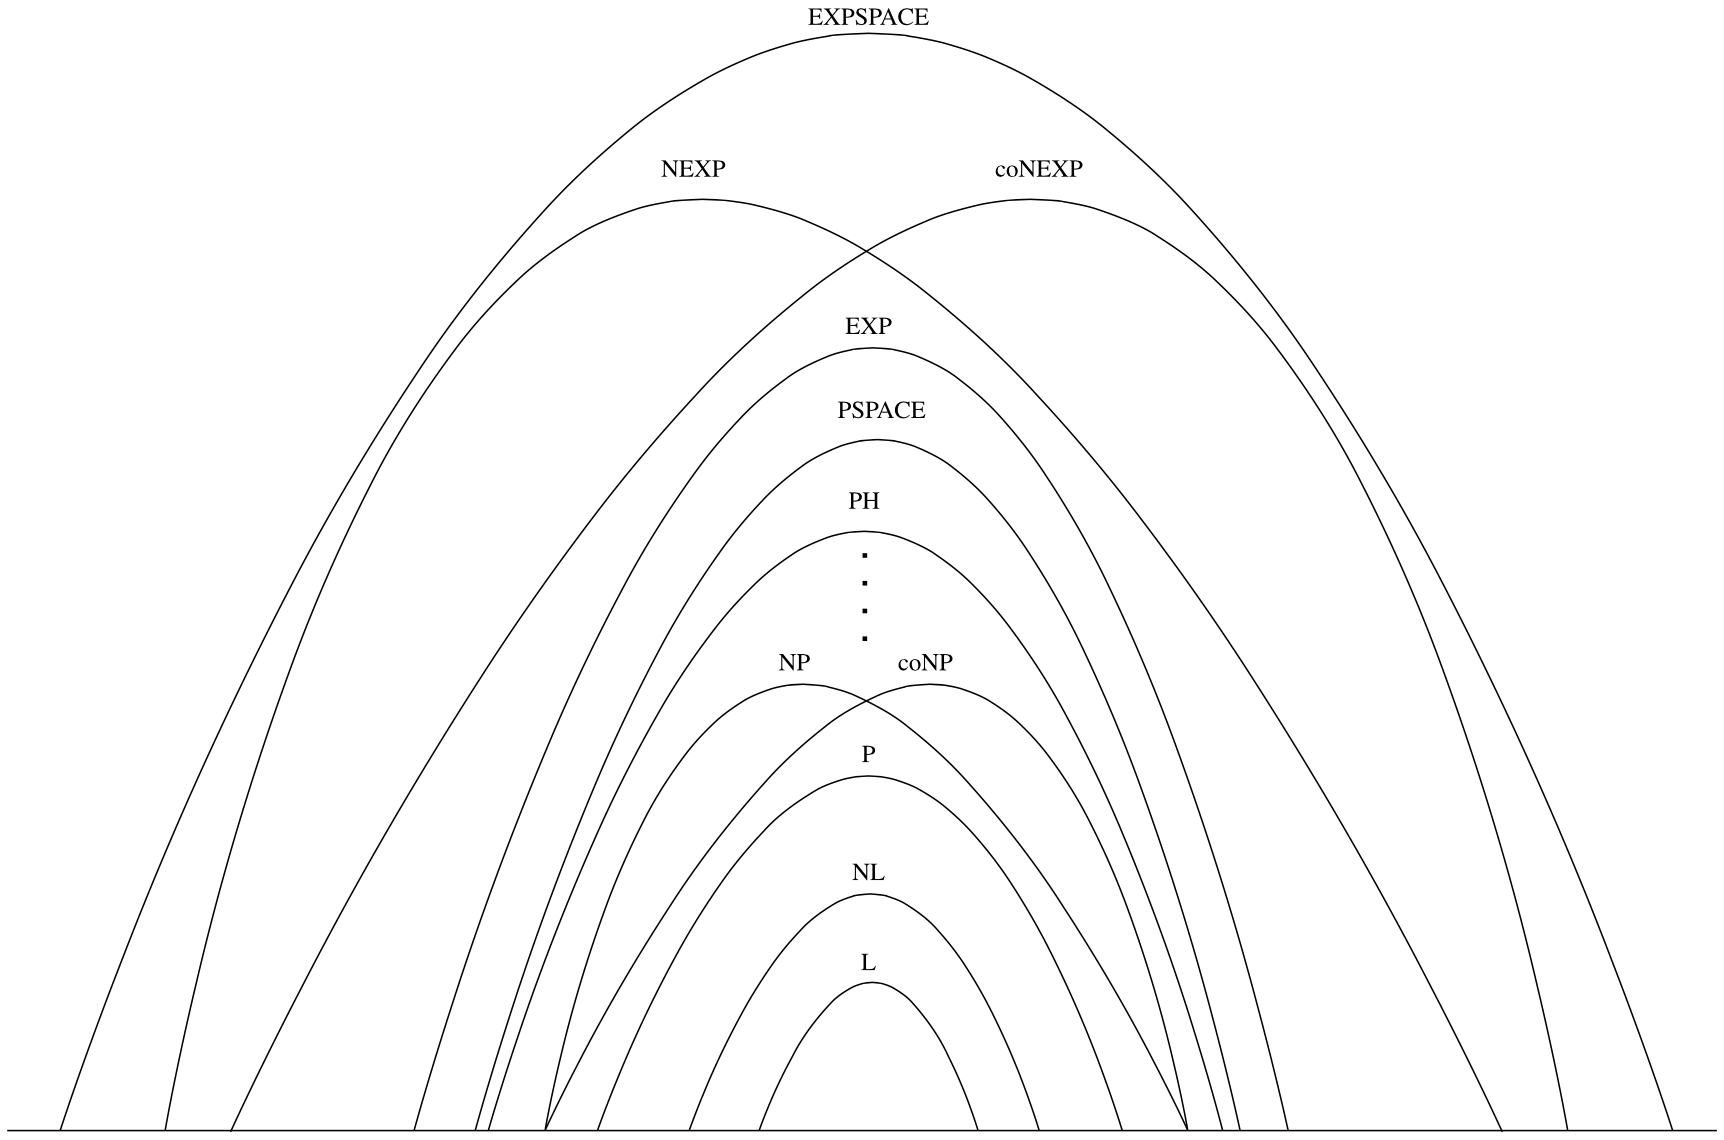
\includegraphics[width=10cm]{img/zoo.png}

Don't worry, in this course you only need to know about P, NP, coNP, and possibly PSPACE.
\end{figure}
\end{frame}

\begin{frame}{here's another zoo.}
We'll call it the \textit{chungus zoo}.

\begin{figure}[h]
\centering
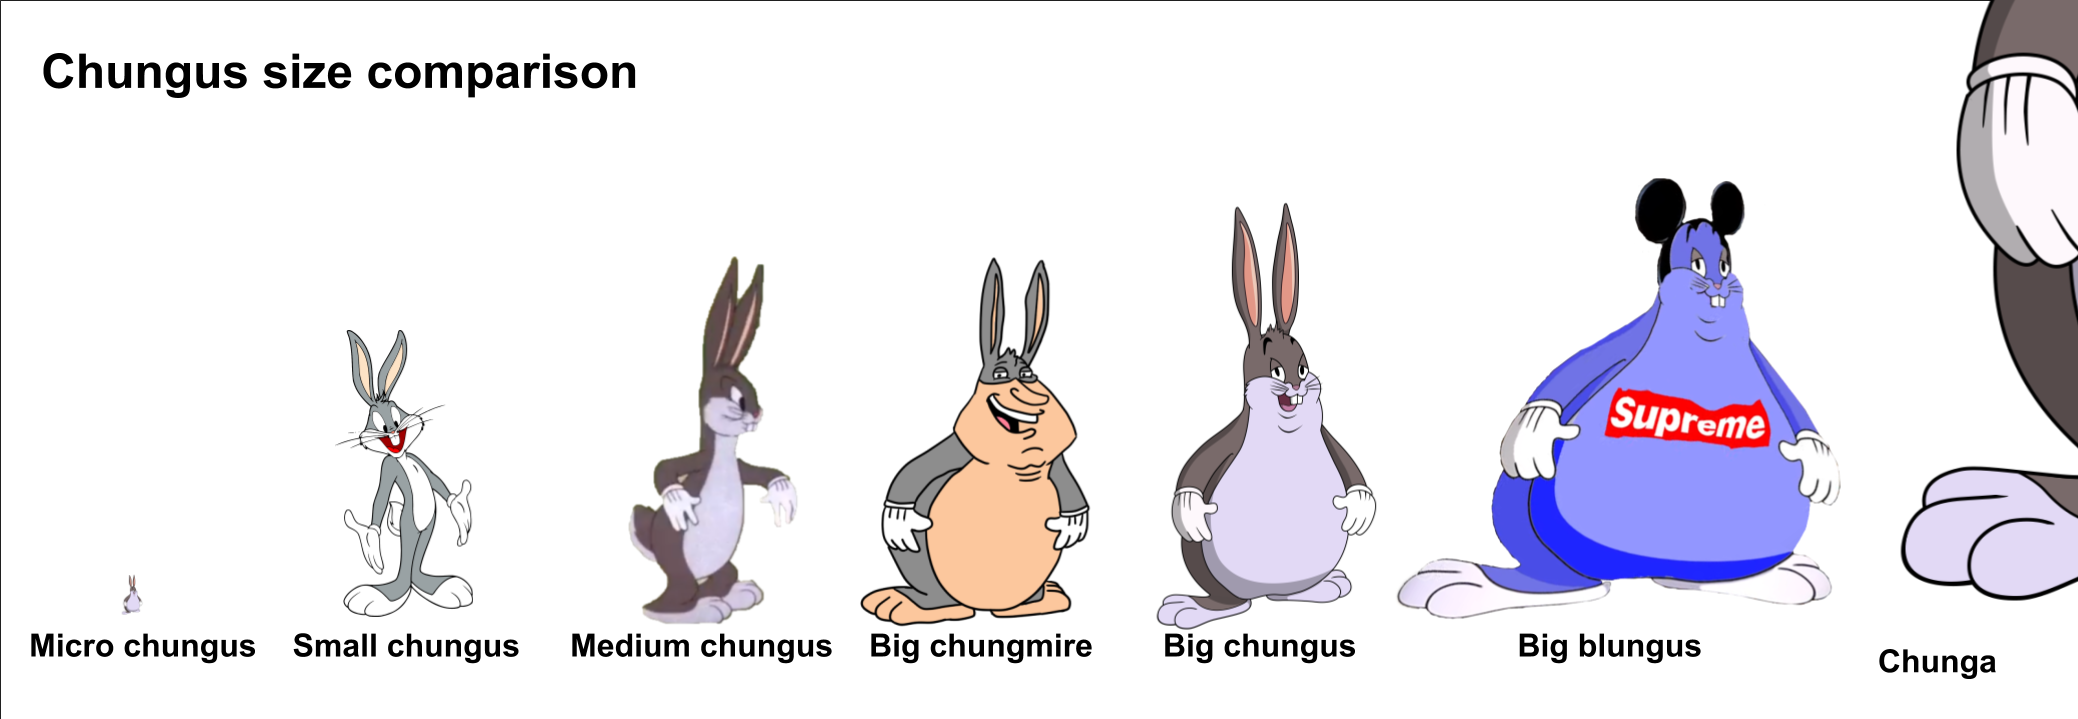
\includegraphics[width=10cm]{img/chungus_sizes.png}

This is what your computer science education has come to.
\end{figure}

Anyway, just like there are many different sizes of chungus, there are many different ``computational complexity'' classes. As you go up the ''computational complexity scale'', you get harder and harder problems. Here's all we know so far:
\begin{align*}
\text{anything practical} \subseteq \text{P} \subseteq \text{NP} \subseteq \text{Decidable} \subseteq \text{Enumerable} \subseteq \Sigma_2 \subseteq \ldots
\end{align*}
(we don't know if $\text P \subsetneqq \text{NP}$.)
\end{frame}

\begin{frame}{verification}
\begin{figure}[h]
\centering

\includegraphics[width=10cm]{img/verify.png}
\end{figure}
\textbf{Question:} Is $221$ a composite number?
\end{frame}

\begin{frame}{verification}
\textbf{Question:} Is $221$ a composite number?

\textbf{Answer:} Yes. $221 = 13 \cdot 17$. (calculator gang)

\vspace{2mm}

\pause

\textbf{Question:} Does $13$ divide $221$?

\textbf{Answer:} Yes.

\vspace{2mm}

\pause

\textbf{Question:} Which of the above two questions is easier to answer?

\textbf{Answer:} Probably the ``does $13$ divide $221$'' one.



\end{frame}

\begin{frame}{verification}
The point is, checking if a number is composite is hard. We can create a TM $M$ that checks if a number is composite:
\begin{align*}
M(x): &\text{For all integers $1 < i < x$:}\\
&\quad \text{If $i$ divides $x$:}\\
&\quad \quad \text{Accept.}\\
&\text{Reject.}
\end{align*}

We can be more efficient with a NTM $M$:
\begin{align*}
M(x): &\text{Nondeterministically choose an integer $1 < i < x$:}\\
&\quad \text{If $i$ divides $x$:}\\
&\quad \quad \text{Accept.}\\
&\text{Reject.}
\end{align*}

\end{frame}

\begin{frame}{verification}
To check if a number $x$ is composite, you're gonna have to go through all integers from $2$ to $x - 1$. But \textit{verifying} that a number $x$ is composite, given a potential factor is easier.

\pause

\vspace{2mm}

Recall the Hamiltonian path problem: Given a graph $G$, to check that it has a H-path would require going through all permutations of the vertices, while it is easier to verify that a given permutation of vertices defines a valid Hamiltonian path.

\pause

\vspace{2mm}

Given a language $A$, a \textbf{verifier} $V$ of $A$ is a Turing machine such that
$$A = \{w: \text{$V$ accepts $(w, c)$ for some string $c$}\}.$$

\end{frame}

\begin{frame}{verification}
Given a language $A$, a \textbf{verifier} $V$ of $A$ is a (deterministic) Turing machine such that
$$A = \{w: \text{$V$ accepts $(w, c)$ for some string $c$}\}.$$

\vspace{2mm}

For example, let $$A = \{x: \text{$x$ is a binary string that corresponds to a composite number}\}.$$

Define $V$ to be the following TM:
\begin{align*}
V(x, y): &\text{If $1 < y < x$ and $y$ divides $x$}:\\
&\quad \text{Accept}\\
&\text{Reject}
\end{align*}
Then $x \in A$ if and only if $V(x, y)$ accepts for some $y$. So
$$A = \{x: \text{$V$ accepts $(x, y)$ for some string $y$}\}$$
meaning $V$ is a verifier for $A$.

\textbf{Task:} Make sense of this.


\end{frame}

\begin{frame}{verification}
Nice theorem! (Go read Sipser's book.)

\begin{theorem}
A language $A$ is in NP if and only if it has a poly-time verifier.
\end{theorem}

(in fact, I think Sipser's book uses existence of poly-time verifier as the \textit{definition} of NP, and then shows $\text{NP} = \bigcup_{k = 1}^\infty \text{NTIME}(n^k)$.)

\end{frame}

\begin{frame}{verification}
fun fact! we can actually determine if a number is prime in poly-time. Search up the ``AKS Primality Test''.

\vspace{2mm}

Not so fun fact: nobody actually uses the AKS primality test, because it's like $O(n^{13})$ or something (which is still polynomial, but impractical!)

\vspace{2mm}

Fun reading: \url{https://en.wikipedia.org/wiki/Galactic_algorithm}

\begin{figure}[h]
\centering

\includegraphics[width=5cm]{img/bye.jpg}
\end{figure}

\end{frame}


\end{document}